\subsubsection{Интерполяция на треугольном КЭ}
\paragraph{Наивный метод}
Рассмотрим треугольник на Рисунке \ref{trig}.
\begin{figure}[H]
	\centering
	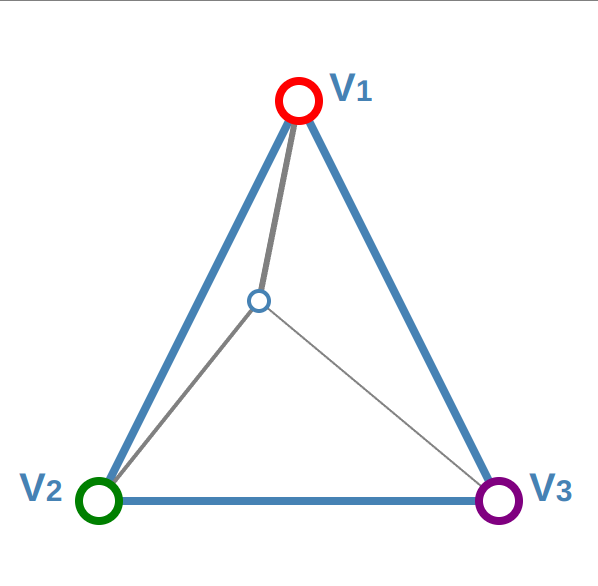
\includegraphics[width=0.4\linewidth,trim={0 0 0 1cm},clip]{img/trig}
	\caption{Треугольник для интерполяции}
	\label{trig}
\end{figure}
Расстояния от точки $P$ до вершин
\begin{align*}
	|P V_1| &= \sqrt{(X_{v1} - P_{x})^2 + (Y_{v1} - P_{y})^2}\\
	|P V_2| &= \sqrt{(X_{v2} - P_{x})^2 + (Y_{v2} - P_{y})^2}\\
	|P V_3| &= \sqrt{(X_{v3} - P_{x})^2 + (Y_{v3} - P_{y})^2}
\end{align*}
Расстояния принимают большие значения, когда точка находимся далеко, и маленькие - когда точка находимся близко. Поэтому инвертируем их, чтобы большие значения придавали больший вес более близким вершинам. Другими словами, мы будем интерполировать обратно пропорционально расстоянию до каждой вершины. \cite{trig_interpolate}
\begin{align*}
	W_{v1} &= 1 - \frac{|P V_1|}{|P V_1|+|P V_2|+|P V_3|}\\
	W_{v2} &= 1 - \frac{|P V_2|}{|P V_1|+|P V_2|+|P V_3|}\\
	W_{v3} &= 1 - \frac{|P V_3|}{|P V_1|+|P V_2|+|P V_3|}
\end{align*}
Это решение простое, его легко начать использовать и оно достаточно интуитивно понятно. Но оно даёт не очень хорошие результаты, если треугольник для интерполяции оказывается вытянутым (см. Рисунок \ref{tri-int-naive-slant}). 
\begin{figure}[H]
	\centering
	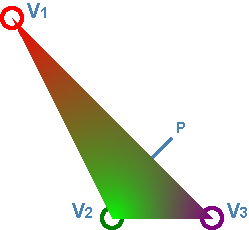
\includegraphics[width=0.45\linewidth]{img/tri-int-naive-slant}
	\caption{Интерполяция значений в треугольном КЭ с помощью наивного метода}
	\label{tri-int-naive-slant}
\end{figure}
На Рисунке \ref{tri-int-naive-slant} видно, что точка $P$, которая находится на ребре $V_1 V_3$ будет иметь значение ближе к значению в вершине $V_2$, что является не совсем правильным поведением алгоритма. В такой точке $P$ хотелось бы получить смесь значений из точек $V_1$ и $V_3$ без $V_2$. 
Код программы для наивного метода:
\lstinputlisting[language=C++, firstline=6, lastline=30]{current-lines/src/Element/GenericElement.cpp}
Перейдём к другому методу интерполяции в треугольном КЭ.

\paragraph{Метод на основе барицентрических координат}
Суть метода барицентрических координат в нахождении барицентрических координат точки $W_{v1}, W_{v2}, W_{v3}$ на основе заданных вершин $V_1, V_2, V_3$, удовлетворяющих системе уравнений \eqref{bary_cases}. \cite{trig_interpolate}
\begin{equation}\label{bary_cases}
	\begin{cases}
		P_x = W_{v1}X_{v1} + W_{v2}X_{v2} + W_{v3}X_{v3},\\
		P_y = W_{v1}Y_{v1} + W_{v2}Y_{v2} + W_{v3}Y_{v3},\\
		W_{v1} + W_{v2} + W_{v3} = 1.
	\end{cases}
\end{equation}

Решение системы \eqref{bary_cases} имеет вид:
\begin{equation*}
	\begin{cases}
		W_{v1}=\dfrac{(Y_{v2}-Y_{v3})(P_{x}-X_{v3})+(X_{v3}-X_{v2})(P_{y}-Y_{v3})}{(Y_{v2}-Y_{v3})(X_{v1}-X_{v3})+(X_{v3}-X_{v2})(Y_{v1}-Y_{v3})},\\[15pt]
		W_{v2}=\dfrac{(Y_{v3}-Y_{v1})(P_{x}-X_{v3})+(X_{v1}-X_{v3})(P_{y}-Y_{v3})}{(Y_{v2}-Y_{v3})(X_{v1}-X_{v3})+(X_{v3}-X_{v2})(Y_{v1}-Y_{v3})},\\[15pt]
		W_{v3}=1 - W_{v1} - W_{v2}.
	\end{cases}
\end{equation*}

Результаты можно увидеть на Рисунке \ref{bary_results}. Видно (см. Рисунок \ref{bary_example}), что теперь при получении значений в точках на ребрах не участвуют значения противолежащих вершин.
\begin{figure}[H]
	\hfill
	\begin{subfigure}{0.48\textwidth}
		\centering
		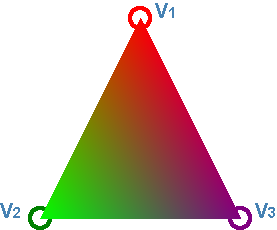
\includegraphics[width=\linewidth]{img/tri-int-bary}
		\caption{Интерполяция значений в треугольном КЭ с помощью метода на основе барицентрических координат}
		\label{tri-int-bary}
	\end{subfigure}
	\hfill
	\begin{subfigure}{0.45\textwidth}
		\centering
		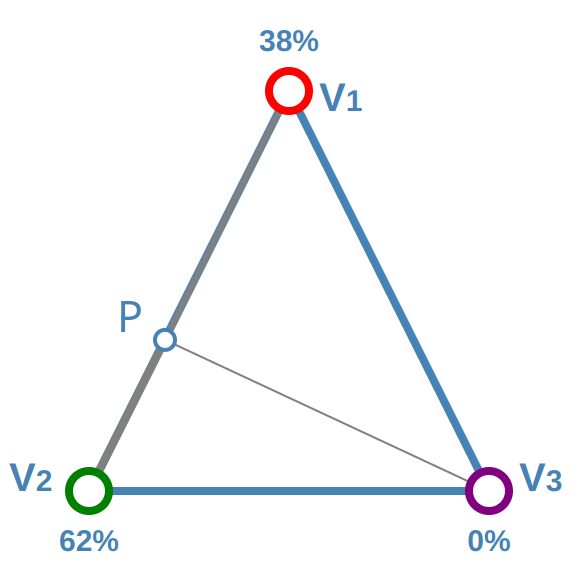
\includegraphics[width=\linewidth]{img/bary_example}
		\caption{Пример интерполяции методом на основе барицентрических координат для точки, лежащей на ребре треугольника}
		\label{bary_example}
	\end{subfigure}
	\hfill
	\caption{Результаты применения метода барицентрических координат}
	\label{bary_results}
\end{figure}
Таким образом метод барицентрических координат работает более точно.
